\documentclass[a4paper,12pt]{report}
\usepackage[left=2cm,right=2cm,top=2cm,bottom=2cm]{geometry}
\usepackage[utf8]{inputenc}
\usepackage{graphicx}
\usepackage{eso-pic}
\usepackage{transparent}
\usepackage{xcolor}
\usepackage{floatrow}
\usepackage{tabularx}
\usepackage{listings}
\usepackage{xcolor}
\usepackage{caption}

\newcommand{\LogoPath}{RUET_logo.png}

\definecolor{odp-background}{RGB}{40, 44, 52}
\definecolor{odp-text}{RGB}{171, 178, 191}
\definecolor{odp-keyword}{RGB}{249, 38, 114}
\definecolor{odp-comment}{RGB}{98, 114, 164}
\definecolor{odp-string}{RGB}{152, 195, 121}
\definecolor{odp-number}{RGB}{174, 129, 255}
\definecolor{odp-function}{RGB}{189, 147, 249}

\lstdefinestyle{cppstyle}{
    language=C++,
    basicstyle=\color{odp-text}\ttfamily\small,
    keywordstyle=\color{odp-keyword},
    commentstyle=\color{odp-comment},
    stringstyle=\color{odp-string},
    numbers=left,
    numberstyle=\tiny\color{odp-number},
    stepnumber=1,
    numbersep=5pt,
    backgroundcolor=\color{gray!5},
    frame=single,
    rulecolor=\color{odp-text},
    breaklines=true,
    breakatwhitespace=true,
    tabsize=4,
    moredelim=[s][\color{odp-header}]{\#include\ <}{>}, % Header files included in #include <>
    otherkeywords={!,!=,~,$,*,\&,\%,:,\#, ifndef, define, endif, include},
    emph={!,!=,~,$,*,\&,\%,:,\#},
    emphstyle=\color{odp-function}
}

\begin{document}
\begin{titlepage}
    \begin{center}

        \AddToShipoutPicture*{\put(0.125\paperwidth,0.125\paperheight){
                \transparent{0.1}
                \includegraphics*[width=0.75\paperwidth,height=0.75\paperheight,keepaspectratio]{RUET_logo.png}%
            }
        }
        \textbf{\textcolor{yellow}{\rmfamily Haven's Light is Our Guide}}

        \begin{figure}[h]
            \transparent{0.8}
            \centering
            \includegraphics[width=0.3\textwidth]{\LogoPath}
        \end{figure}

        \vspace*{0in}
        \Large
        \textbf{\mbox{Rajshahi University of Engineering \& Technology}}
        \large
        \textbf{\mbox{\textcolor{blue}{Department of Computer Science \& Engineering}}}

        \vfill
        \Huge
        \textbf{\mbox{Lab Report}}
        \vfill

        \begin{table}[h]
            \centering
            \begin{tabularx}{0.7\paperwidth}{|c|X|}
                \hline
                \textbf{Course Code:}     & CSE 2204                                                                                                                  \\
                \hline
                \textbf{Course Title:}    & Numerical Methods Sessional                                                                                               \\
                \hline
                \textbf{Experiment No:}   & 01                                                                                                                        \\
                \hline
                \textbf{Experiment Name:} & Solving Algebric and Transcendental Equations using Bisection and False Position Method and Comparison of their Efficency \\
                \hline
            \end{tabularx}%
        \end{table}

        \vspace{0.5in}
        \textbf{Date:} \\
        \today

        \vfill

        \begin{table}[h]
            \centering
            \begin{tabularx}{0.7\paperwidth}{|X|X|}
                \hline
                Submitted By:               & Submitted To:                                    \\
                \hline
                Name: Md. Abdullah Al Mamun & Shyla Afroge                                     \\
                \hline
                Section: A                  & Assistant Professor                              \\
                \hline
                Roll No: 2003028            & Computer Science \& Engineering                  \\
                \hline
                Year: 2nd Year Odd Semester & Rajshahi University of Engineering \& Technology \\
                \hline
            \end{tabularx}
        \end{table}
    \end{center}
\end{titlepage}

\section*{Experiment No: 01}
\section*{Experiment Name: \small Solving Algebric and Transcendental Equations using Bisection and False Position Method and Comparison of their Efficency}
\section*{Theory:}

\subsection*{Bisection Method:}
\qquad The bisection method is a numerical approach employed for finding the root of a real-valued function within a specified interval. The method begins by selecting an initial interval $[a, b]$ such that the function has opposite signs at the endpoints ($f(a) \cdot f(b) < 0$), adhering to the Intermediate Value Theorem. The process iteratively narrows down the interval by evaluating the function at the midpoint $c = \frac{a+b}{2}$. If $f(c) = 0$, $c$ is the root; otherwise, the interval containing the root is determined based on the signs of $f(a)$ and $f(c)$. This iterative process continues until the interval becomes sufficiently small or a predetermined number of iterations is reached, ensuring convergence. While the bisection method is straightforward and guaranteed to converge, it may converge slowly for certain functions due to its halving of the interval at each step. Nevertheless, its reliability and simplicity make it a widely used numerical technique in various scientific and engineering applications.

\subsection*{Algorithm:}
\begin{enumerate}
    \item Interval Selection: Choose an initial interval $[a, b]$ such that the function has opposite signs at the endpoints ($f(a) \cdot f(b) < 0$), adhering to the Intermediate Value Theorem.
    \item Iterative Process: Divide the interval in half and evaluate the function at the midpoint $c = \frac{a+b}{2}$. If $f(c) = 0$, $c$ is the root. Otherwise, determine the subinterval $[a, c]$ or $[c, b]$ in which the root must lie based on the signs of $f(a)$ and $f(c)$ (or $f(b)$ and $f(c)$).
    \item Convergence Criteria: Repeat the process iteratively until the interval becomes sufficiently small or until a predetermined number of iterations is reached. The Bisection method converges to the root because it progressively narrows down the interval containing the root.
    \item Accuracy Improvement: The accuracy of the root approximation improves with each iteration, and the method typically converges linearly. The precision can be controlled by specifying a tolerance level or a maximum number of iterations.
\end{enumerate}

\subsection*{False Position Method:}
\qquad The False Position method, also known as the Regula Falsi method, is a numerical technique used for approximating the root of a real-valued function within a specified interval. Similar to the bisection method, it relies on the Intermediate Value Theorem, but instead of bisecting the interval, it employs linear interpolation between function values. The method iteratively updates the interval based on the function values at the endpoints, aiming to reduce the width of the interval containing the root. The False Position method can converge faster than the bisection method, but it may encounter convergence issues if the initial interval is poorly chosen or if the function exhibits erratic behavior. Despite these considerations, the method remains a valuable tool for numerical root-finding, particularly when a faster convergence rate is desired.

\subsection*{Algorithm:}
\begin{enumerate}
    \item Interval Selection: Choose an initial interval $[a, b]$ such that the function has opposite signs at the endpoints ($f(a) \cdot f(b) < 0$), adhering to the Intermediate Value Theorem.
    \item Linear Interpolation: Interpolate linearly between function values at the endpoints to find the point $c$ where the line intersects the x-axis. Evaluate $f(c)$.
    \item Interval Update: Determine the subinterval $[a, c]$ or $[c, b]$ in which the root must lie based on the signs of $f(a)$ and $f(c)$ (or $f(b)$ and $f(c)$).
    \item Convergence Criteria: Repeat the process iteratively until the interval becomes sufficiently small or until a predetermined number of iterations is reached. The False Position method aims to reduce the width of the interval containing the root.
    \item Accuracy Improvement: The accuracy of the root approximation improves with each iteration, and the method typically converges faster than the Bisection method. However, it may encounter convergence issues if the initial interval is poorly chosen or if the function exhibits erratic behavior.
\end{enumerate}

\section*{Program:}

\begin{lstlisting}[style=cppstyle, caption={Bisection Method}, label={lst:cppcode}, basicstyle=\fontsize{10}{11}\selectfont\ttfamily]
    double rootByBisection(double a, double b, bool print = false)
    {
        int i = 0;
        double error = abs(a - b), c;

        while (abs(error) > 0.0001)
        {
            if (print)
                cout << i + 1 << "\t|\t" << a << "\t|\t" << b << "\t|\t" << c << "\t\t|\t" << function(c) << "\t\t|\t" << error << "\n";

            c = (a + b) / 2;
            if (function(a) * function(c) < 0)
                b = c;
            else
                a = c;

            error = abs(a - b);

            if (i > MAX_ITERATION)
                break;
            i++;
        }
        return c;
    }
\end{lstlisting}

\begin{lstlisting}[style=cppstyle, caption={False Position Method}, label={lst:cppcode}, basicstyle=\fontsize{10}{11}\selectfont\ttfamily]
    double rootByFalsePosition(double a, double b, bool print = false)
    {
        int i = 0;
        double c;

        while (abs(function(c)) > 0.0001)
        {
            if (print)
                cout << i + 1 << "\t|\t" << a << "\t|\t" << b << "\t|\t" << c << "\t\t|\t" << function(c) << "\t\t|\t" << function(c) * 100 << "%\n";

            c = b - function(b) * (b - a) / (function(b) - function(a));

            if (function(a) * function(c) < 0)
                b = c;
            else
                a = c;

            if (i > MAX_ITERATION)
                break;
            i++;
        }
        return c;
    }
\end{lstlisting}

\begin{lstlisting}[style=cppstyle, caption={Main Program}, label={lst:cppcode}, basicstyle=\fontsize{10}{11}\selectfont\ttfamily]
    #include <iostream>
    #define MAX_ITERATION 100
    using namespace std;

    double function(double x)
    {
        return x * x * x - 2 * x - 5;
    }

    int main()
    {
        int choice;
        double a = -1, b = 1;

        while (function(a) * function(b) > 0)
        {
            function(b) > function(a) ? b++ : a--;
        }

        // cout << "a: " << a << "\tb: " << b << "\n";

        cout << "Menu Program: \n";
        cout << "\t1. Bisection Method\n";
        cout << "\t2. False Position Method\n";
        cout << "\t3. Compare Both Methods\n";
        cout << "Enter Your Choice: ";
        cin >> choice;

        cout << "\n\nn\t|\ta\t|\tb\t|\tx\t\t|\tf(x)\t\t|\terror\n";
        cout << "---------------------------------------------------------\n";

        switch (choice)
        {
        case 1:
            rootByBisection(a, b, true);
            break;
        case 2:
            rootByFalsePosition(a, b, true);
            break;
        case 3:
            cout << "Bisection Method: " << rootByBisection(a, b) << " with error: " << function(rootByBisection(a, b)) * 100 << "%\n";
            cout << "False Position Method: " << rootByFalsePosition(a, b) << " with error: " << function(rootByFalsePosition(a, b)) * 100 << "%\n";
            break;
        }
    }
\end{lstlisting}

\section*{Result:}
\qquad The Bisection and False Position methods are numerical techniques employed for finding the roots of a real-valued function. In the Bisection method, the interval containing the root is successively halved until a sufficiently accurate root approximation is achieved. While it guarantees convergence, it may be slow for certain functions. On the other hand, the False Position method, also known as the Regula Falsi method, utilizes linear interpolation between function values to approximate the root. Although it typically converges faster than Bisection, it can encounter convergence issues if the initial interval is poorly chosen or if the function exhibits erratic behavior. Both methods have their strengths and limitations, with the choice between them often dependent on the specific characteristics of the function being analyzed.

\begin{figure}[H]
    \centering
    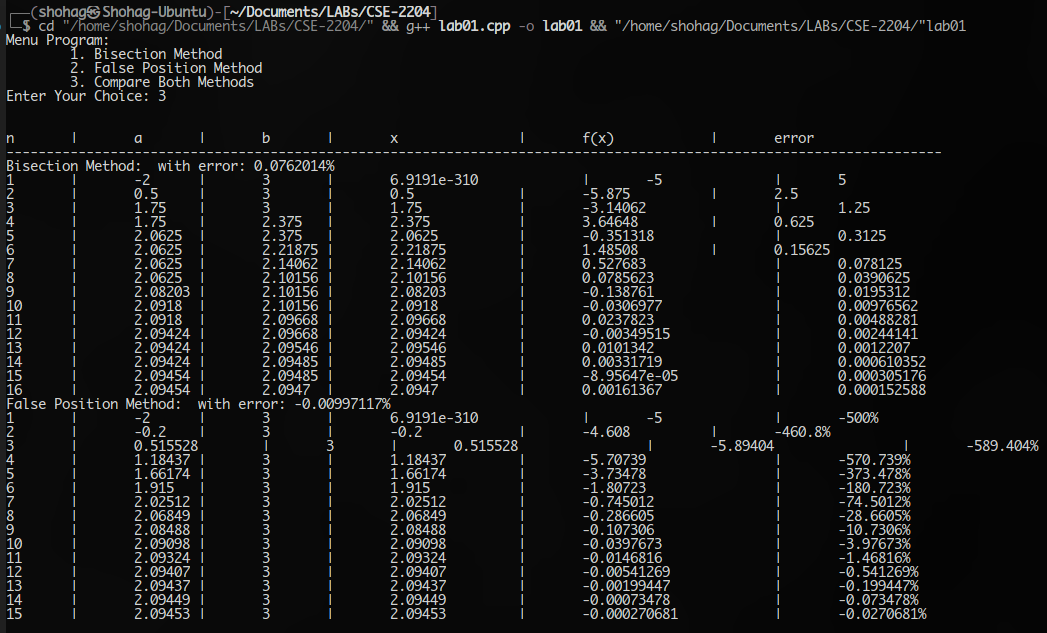
\includegraphics[width=\textwidth]{result.png}
    \caption{Output of the Program}
    \label{fig:result}
\end{figure}

\end{document}